\chapter{Metallic Bonds: Why Copper Can Be Drawn into Wire}

\begin{kaichang}
\textbf{Translator safety note:} Do not try the glass-breaking comparison below. Observe a teacher's example or use the stated chalk alternative with adult supervision and eye protection; keep fragments away from your face. See \href{https://www.acs.org/education/celebrating-chemistry-editions/2024-ccew/science-safety-tips.html}{ACS activity safety guidance}.

Find a piece of discarded electrical wire and ask an adult to remove its plastic covering (inspect it only; do not connect it to power). Inside is a bundle of reddish strands: copper wire. Bend one by hand. It bends and stays bent, neither breaking nor springing back. Now try a glass rod or chalk stick of roughly similar thickness: snap---it breaks.

Consider what that copper wire does. A factory draws a large copper billet into wire finer than hair, kilometers long without breaking it into pieces. Wrapped in plastic and connected to electricity, it lights lamps and charges phones. Both are solids made of atoms, so why can copper be drawn almost endlessly into wire and let current pass freely, while glass and chalk break when bent and ``play dead'' electrically?

Do not rush to answer ``because copper is a metal.'' That merely renames the question. The real question is: how exactly do atoms inside metals hold together? This chapter magnifies that wire all the way down to the atomic level.
\end{kaichang}

\section{Metals' Four Shared Faces}

Line up the world's eighty-plus metals: iron, copper, aluminum, gold, silver, tin, zinc, nickel, titanium, and more. They differ in color, hardness, and price, but nearly all share four faces.

First: \textbf{electrical conduction}. Household wiring uses copper, high-voltage transmission lines aluminum, and socket spring contacts copper alloys. Nearly every route for electricity is entrusted to metals, while plastic, ceramics, glass, and dry wood ``block'' it.

Second: \textbf{heat conduction}. Woks are iron or aluminum because heat must travel quickly from the bottom into food. Handles must instead be wood or plastic, or your hand joins the meal. In winter, a table's iron legs feel colder than its wooden top. Keep that detail in mind; it matters at the chapter's end.

Third: \textbf{deformation without shattering}. Copper draws into fine wire; aluminum rolls into foil thinner than paper; gold is more extreme still: one gram can be hammered into nearly a square meter of leaf, thin enough to transmit light. Craftspeople call this ``malleability and ductility.'' Repeatedly bend a paper clip and it hardens before finally breaking. Salt crystals, glass, and ceramics crack with only a slight bend. These two ways of ``dying'' are entirely different, and the comparison will prove crucial.

Fourth: \textbf{metallic luster}. Freshly cut metals shine. Gold, silver, and platinum have made jewelry of this property for millennia. Powdered aluminum and silver in paint make ``silver paint''; deposited behind glass, they make mirrors.

Four traits across eighty-plus otherwise different elements. Chapter 10 said common traits in the periodic table must share a cause. Copper, iron, and aluminum hold no meetings, so how do they agree? The trail leads back to electrons.

\begin{shiyan}
\textbf{Translator safety note:} The LED circuit below is incomplete without proper current limiting. A metal test object is not an adequate substitute for a rated series resistor. Have a knowledgeable adult select the resistor for the actual LED and supply before connecting anything; never short a battery. See \href{https://www.kingbrightusa.com/applicationnotes/ApplicationNotesFor_SMD_LEDs.pdf}{Kingbright's LED application notes} and \href{https://oem.energizer.com/english/dos-donts/}{Energizer's battery precautions}.

\textbf{Materials}: a 9-volt battery (or two AA batteries in series), an LED or small torch bulb, and several wires. Test objects: a metal key, coin, pencil lead (removed from a pencil or a mechanical-pencil refill), plastic ruler, eraser, folded aluminum foil, and paper clip.

\textbf{Procedure}:
\begin{enumerate}[itemsep=1pt]
\item Connect the battery, LED, and wires into a circuit with a deliberate gap. The LED's long leg should face the battery's positive terminal.
\item Use each object to ``bridge'' the gap, touching its ends to the two loose wire ends. Record whether the LED lights in two columns: on / off.
\item Try a ``bending test'': straighten the paper clip and bend it repeatedly, feeling the changes. Then gently bend a chalk stick and observe what happens.
\end{enumerate}

\textbf{What to observe}: which objects light the LED? Pencil lead conducts too, though it is graphite rather than metal. Chapter 24 explores this ``nonmetal exception.'' Does the paper clip become hot and hard before breaking? How does chalk's ``death'' differ?

\textbf{Safety note}: use batteries only, at no more than 9 volts. \textbf{Never} experiment with mains electricity from an outlet. Do not leave the LED connected directly across the battery for long; put a test object or small resistor in series to avoid burning it out.
\end{shiyan}

\section{Zooming In: A City in an Electron Sea}

Recall Chapters 10 and 11: metals occupy the periodic table's left and middle, sharing \textbf{few outer electrons that are relatively distant from the nucleus and loosely bound}. Sodium has 1 outer electron, magnesium 2, aluminum 3; even transition metals such as iron and copper have outer electrons that are not particularly settled.

Imagine countless copper atoms packed together. Each outer electron is already only moderately attracted to its own nucleus, and neighboring nuclei now crowd around it. Energetically, ``staying home'' and ``visiting next door'' are nearly equivalent. The outer electrons therefore \textbf{cease to belong to any particular atom}, becoming the whole block's ``public property,'' free to wander throughout it.

What remains? Metal atoms missing their outer electrons become positive \textbf{cations}, arranged regularly like fixed buildings in a carefully planned city. The free electrons immerse the city like seawater.

\begin{center}
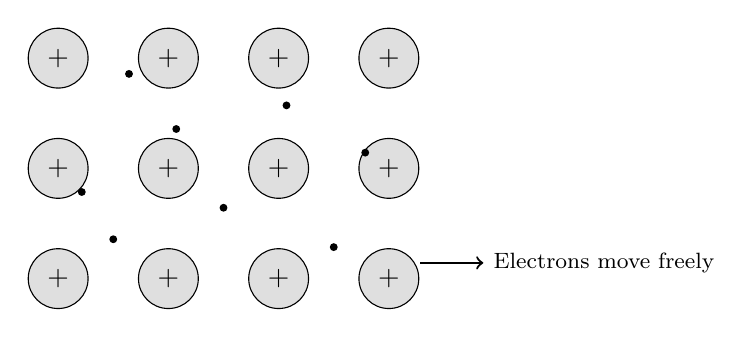
\begin{tikzpicture}
\foreach \x in {0,1.4,2.8,4.2} {
  \foreach \y in {0,1.4,2.8} {
    \draw[fill=gray!25] (\x,\y) circle (0.38);
    \node at (\x,\y) {$+$};
  }
}
\fill (0.7,0.5) circle (0.05);
\fill (2.1,0.9) circle (0.05);
\fill (3.5,0.4) circle (0.05);
\fill (0.3,1.1) circle (0.05);
\fill (1.5,1.9) circle (0.05);
\fill (2.9,2.2) circle (0.05);
\fill (3.9,1.6) circle (0.05);
\fill (0.9,2.6) circle (0.05);
\draw[->,thick] (4.6,0.2) -- (5.4,0.2) node[right]{\footnotesize Electrons move freely};
\end{tikzpicture}

\footnotesize A representation of a metal's interior: large circles are fixed metal cations; small dots are roaming delocalized electrons. Circles, proportions, and positions do not show its actual appearance.
\end{center}

This is \textbf{metallic bonding}: not sticks joining pairs of atoms (Chapter 17 dismantled that metaphor), but electrical attraction between ``orderly cations'' and a ``flowing electron sea.'' Negative electrons attract positive cations, binding the whole metal into a lower-energy system. The general account---forming bonds releases energy, breaking them absorbs it---is the same as for every chemical bond in Chapter 17.

Compare its neighbors from earlier chapters. In ionic bonding (Chapter 18), electrons are \textbf{transferred} outright to atoms such as chlorine, staying with their new owner. In covalent bonding (Chapter 19), two atoms \textbf{jointly own} electrons within the small region between their nuclei. In metallic bonding, electrons are \textbf{publicly owned by everyone}, roaming the whole block. Chemists call this belonging to the entire system rather than a particular atom pair \textbf{delocalization}. All three bonds fundamentally involve attraction between charges; their difference lies in electrons' ``residency rules'': private, joint, or public ownership.

\section{One Model Explains All Four Faces}

The picture of ``cations in an electron sea'' is astonishingly powerful: it explains all four shared metallic traits at once.

\textbf{Electrical conduction}: the sea is full of mobile charged particles. Normally they wander randomly like people in a square, going nowhere on average. Connect a battery across the metal and apply an electric field, and their random motion gains a slow directed drift: current. Plastic and glass have no such free electrons. Covalent bonds tie their electrons to particular atom pairs, leaving no troops to dispatch when an electric field arrives.

\textbf{Heat conduction}: a flame beneath a pan makes nearby metal atoms vibrate more vigorously. Free electrons collide with them and acquire energy, then race to distant ions and transfer it onward. The electron sea is a highway for both current and heat. No wonder good electrical conductors are usually good thermal conductors; copper, aluminum, and silver excel at both.

\textbf{Ductility and malleability}: this is metallic bonding's proudest performance. Hammering makes orderly cation layers slide past one another. In an ionic crystal like Chapter 18's salt, sliding turns alternating neighbors into positive-facing-positive and negative-facing-negative. Repulsion shatters the crystal, so salt and glass break when bent. Metals need not fear this: as cation layers slide, the electron sea immediately fills the new spaces and keeps binding the positive ions. Metallic bonds are \textbf{nondirectional}, unconcerned with neighbors' precise positions, so sliding does not break them. That is why copper can become kilometers of fine wire.

\textbf{Luster}: free electrons can also absorb incoming light of many colors and ``spit it back'' almost unchanged. A metal surface thus shines like an electron-built mirror. Copper looks reddish and gold yellowish because their reflection efficiencies differ slightly with color, for deeper quantum reasons.

\begin{qiaoliang}
How many ``free electrons'' are there, and how fast do they move? Copper's density is about \ud{8.9}{g/cm^3} and its molar mass about \ud{64}{g/mol}. Thus \ud{1}{cm^3} contains about $8.9\div 64\approx 0.14$ moles of atoms, or $0.14\times 6.02\times 10^{23}\approx 8.4\times 10^{22}$ atoms. With one outer electron per atom entering the sea, a sugar-cube-sized piece contains $8.4\times 10^{22}$ free electrons---ten trillion times Earth's population.

Now their speed in a current. Suppose a copper wire with cross section \ud{1}{mm^2} carries \ud{1}{A}, roughly a small desk lamp's current. Using current = electron density × charge × drift speed × cross-sectional area gives about $7\times 10^{-5}$ \ud{}{m/s}, or \textbf{about 0.07 millimeters per second}---dozens of times slower than a snail! Yet a lamp lights the instant you flip its switch. Why? The ``start'' signal is not an electron traveling from switch to bulb. An electric field spreads along the wire at nearly light speed, telling electrons \textbf{already present everywhere} to start drifting together. A wire never waits for electrons to ``arrive''; its city is already fully populated.
\end{qiaoliang}

\section{Symbols: Substances Without ``Molecular Formulas''}

Now for symbols: copper \chem{Cu}, iron \chem{Fe}, aluminum \chem{Al}, silver \chem{Ag}, gold \chem{Au}. Notice that a metal's ``formula'' is simply its element symbol. This is not laziness but a statement of fact. A copper block contains no identifiable ``copper molecules''; it is one enormous whole of countless \chem{Cu} atoms (more precisely, \chem{Cu} cations plus an electron sea), whose smallest ``structural unit'' is the atom. Salt is similar: Chapter 18 explained that \chem{NaCl} denotes an ionic ratio, not isolated salt molecules. Metals do not even need a ratio: their city has just one kind of resident.

Because metals contain no molecules, ``a copper molecule'' makes the same mistake as ``a salt molecule.'' This is convenient in calculations: \ud{64}{g} of copper is 1 mole of copper atoms, with no middleman.

\section{How Scientists Know: The Electron Sea Was Not Made Up}

\begin{zhengju}
``An electron sea inside metals'' sounds like a clever story. Why believe it? Evidence came from an elegant ``cross-disciplinary reconciliation.''

In 1853, the German physicists Wiedemann and Franz measured electrical and thermal conduction in many metals. They found a remarkable pattern: at the same temperature, \textbf{thermal conductivity divided by electrical conductivity was nearly constant across metals}, and this ratio increased proportionally with temperature. Silver, copper, iron, and lead differed so greatly, yet their ratios seemed coordinated. This suggested that \textbf{the same carriers} transported electricity and heat. Two unrelated sets of particles would have no reason to yield such consistent ratios.

In 1900, only three years after the electron's discovery (Thomson's experiment from Chapter 7), Drude formally proposed an internal ``electron gas,'' traveling freely among cations like gas molecules. Calculations reproduced the Wiedemann--Franz ratio, giving the electron-sea model its first solid evidence.

But victory was not the end. Drude's model soon hit a wall. Contemporary statistical physics said that if each atom contributed one free electron, those electrons should absorb heat like gas molecules, making metals' heat capacities substantially larger than those of nonmetal solids. Measurements instead found nearly identical capacities: those hundreds of quintillions of ``free electrons'' seemed absent from heat absorption. A model explaining conduction but not heat capacity had to be missing something.

The correction awaited quantum mechanics. In 1927--1928, Sommerfeld, Bloch, and others recalculated electrons as quantum waves. Electrons in the sea were not equally free: they had to occupy seats from low energy upward, and most were surrounded by occupied seats with nowhere to go. Only a small fraction at the highest energies, close to the ``sea surface'' (the Fermi surface), had empty states available and could actually participate in electrical and thermal conduction. At room temperature, the freely active fraction was on the order of one percent, explaining its barely measurable heat-capacity contribution. The contradiction was resolved and the model upgraded. Scientific models do not become truth upon proposal: they explain some facts, are cornered by new ones, then develop sharper teeth.
\end{zhengju}

\section{From Electron Seas to Bands: Why Copper Conducts and Sulfur Does Not}

The quantum correction also answered a deeper question: why do metals have free electrons while nonmetals do not?

An isolated atom's electrons occupy discrete ``floors'' (Chapter 9). Pack $N$ atoms together and neighbors affect each floor, splitting it into $N$ closely spaced lines. With $N$ on the order of one septillion, the lines merge into a dense region called an \textbf{energy band}. Between bands may lie a forbidden region with no floors, called a \textbf{band gap}.

\begin{itemize}[itemsep=2pt]
\item \textbf{Metals} (copper, iron, aluminum): the outer band is partly empty or overlaps an empty band above. A little extra energy gives electrons nearby vacant states, allowing the electron sea's free movement and conduction of heat and electricity.
\item \textbf{Insulators} (sulfur, glass, diamond): the outer band is full, with a wide gap above it. Nobody in the crowded carriage can move, and ordinary voltages cannot supply enough energy to cross the gap. Electrons are ``welded in place,'' preventing conduction.
\item \textbf{Semiconductors} (silicon, germanium): a narrow gap lets thermal motion or doping move a few electrons across. Conductivity lies between the other two and can be precisely controlled. Your phone's chips rely on this tunability (Chapter 10 introduced silicon in this role).
\end{itemize}

The electron-sea model and band theory are two floors of one building: the first explains what free electrons do; the second explains where they come from and why some materials have none. For middle-school purposes, the sea is enough. We need only crack open the band-theory door and glimpse the light inside.

\section{Moving ``Outsiders'' into the City: Alloys}

Pure metals have a workplace weakness: easy layer sliding generally makes them soft. Pure iron bends by hand, pure aluminum dents under pressure, and pure gold is too soft for rings. For millennia, humans have strengthened metals the same way: \textbf{mix in other atoms to make alloys}.

Metallic bonding explains why. Layers slide easily because they are orderly. Introduce differently sized ``outsiders'': large atoms squeeze into the ranks, while small ones enter gaps. Smooth sliding routes become bumpy and difficult to traverse. Difficult sliding means harder, stronger material. The electron sea still binds everything, so alloys retain electrical conduction and luster.

You have probably eaten with, used, or sat on items from this ``mixed'' menu:

\begin{itemize}[itemsep=2pt]
\item \textbf{Steel}: iron with a little carbon, usually below 2\,\% by mass. Small carbon atoms fit into gaps in the iron array, blocking sliding routes and turning soft iron tough. Bridges, rails, and reinforcing bars rely on this addition. Too much carbon makes it brittle, so steelmaking essentially controls the number of ``stoppers.'' Add chromium (above about 12\,\%) and nickel, and a thin chromium-oxide film makes rust struggle to take hold: stainless steel. We will encounter chromium's ability again in Chapter 15's transition-metal neighborhood.
\item \textbf{Bronze}: copper with tin, humanity's first alloy, which ushered in the ``Bronze Age'' more than three thousand years ago. Harder than copper and lower-melting, it casts readily into ritual vessels, swords, and bells.
\item \textbf{Brass}: copper with zinc. Its golden color often imitates gold in instruments, taps, and cartridge cases. Slightly larger zinc atoms substitute into copper's ranks, also obstructing sliding.
\item \textbf{Aluminum alloys}: aluminum's strength is low density, only a third of iron's; its weakness is softness. A little copper, magnesium, and silicon can give steel-like strength with far less weight---the bargain behind aircraft bodies, drinks cans, and bicycle frames.
\item \textbf{Shape-memory alloys}: nickel and titanium in roughly equal atomic proportions perform a trick: bend them, pour warm water over them, and they return to their original shape. Their atomic lattice switches between two arrangements with temperature, like a drill team remembering two formations. Spectacle frames, orthodontic wires, and cardiovascular stents use this metal that ``remembers itself.''
\end{itemize}

Alloys are not compounds. Iron and carbon, or copper and zinc, have no fixed proportions and no chemical formula. They resemble a carefully proportioned stew, with atoms sharing a lattice and the same electron sea. Their properties can therefore be continuously tuned like recipes, a materials engineer's core skill.

\section{Where This Model Hits Its Limits}

Every model has boundaries, including the electron sea. It excels at \textbf{common traits}: why metals conduct heat and electricity, deform, and shine. But \textbf{individual differences} make it vague:

\begin{itemize}[itemsep=2pt]
\item Why do magnets attract iron, cobalt, and nickel but not copper and aluminum? Magnetism comes from collective electron-spin alignment, absent from this model.
\item Why does tungsten melt at $3422\,^{\circ}\mathrm{C}$, while mercury melts at $-39\,^{\circ}\mathrm{C}$ and is liquid at room temperature? Saying both are ``cations in a sea'' cannot explain nearly three and a half thousand degrees of difference.
\item Why do some metals lose all resistance near absolute zero, letting current circulate forever (superconductivity)? This needs a quantum picture of paired electrons. Onnes's discovery in 1911 stunned physicists, and even today a complete explanation of high-temperature superconductivity remains unresolved.
\end{itemize}

Quantum mechanics stands behind all these walls. Put this model in its proper place: it is an excellent first pair of glasses for qualitatively explaining metals' four common traits. Predicting a particular metal's hardness, melting point, or magnetism requires finer lenses.

\begin{wuqu}
``Metal feels cold because its temperature is lower than its surroundings.'' A deceptively convincing mistake. Leave iron and wood in the same room overnight and they must reach the same room temperature, as a thermometer confirms. Your fingers, however, are about $33\,^{\circ}\mathrm{C}$, warmer than the room. Wood carries heat away slowly, allowing skin contact points to warm quickly and feel warm. Iron's electron sea rapidly draws heat from your fingertips and spreads it along the bar, keeping your skin cool. ``Cold'' means not lower iron temperature but faster heat loss from you. Reverse the reasoning: a hot iron pan burns more than a wooden spatula at the same temperature because it pours heat into your hand faster. Thermal conductivity describes the \textbf{rate of heat transfer}, not how hot or cold an object is. Rate and amount are always different things.
\end{wuqu}

\section{Back to the Copper Wire}

Now strip that wire again.

Copper can be drawn kilometers long without breaking because its \chem{Cu} cation layers slide during drawing, while the delocalized electron sea instantly fills each new arrangement and binds the city. Metallic bonding is nondirectional: wherever the layers slide is still home. Glass and chalk break because their atoms have directional covalent bonds or alternating ionic bonds; displaced positions turn attraction into repulsion.

Copper conducts because each atom's outer electron becomes public property, with one hundred nonillion free electrons already filling the entire wire. Closing the switch sends an almost light-speed electric-field command, and electrons across the city begin drifting at less than a millimeter per second. The lamp lights immediately, without an electron being ``express-delivered'' from the power station.

What about the plastic covering? Its molecular electrons are tightly bound to particular atom pairs by covalent bonds (Chapter 19), with full carriages and a wide band gap, leaving no free electrons to dispatch. It insulates, protecting you from stray current. A wire is ``electron sea'' and ``private electron ownership'' working side by side: copper lets electrons flow; plastic keeps them from flowing where they should not. Bond type directly determines a material's job.

\section{Looking Ahead to the Next Stop}

This chapter showed a copper block held together by ``cations in an electron sea.'' In Chapter 18, salt crystallizes through attraction between opposite ions; in Chapter 19, water molecules hold their internal atoms together by sharing electrons.

But we have kept skipping a question. Hydrogen and oxygen within water join covalently, but what about \textbf{one water molecule and another}? Water gathers into drops, sugar dissolves, geckos hang from ceilings, and cling film sticks to bowls. Between their molecules lies a ``weak tug,'' insufficient for bonding yet undeniably real. Metallic, ionic, and covalent bonds cannot account for it: they explain how atoms form molecules or crystals, not how molecules get along. What is this weaker attraction that nevertheless shapes the whole world? In Chapter 22, we will catch the hand hidden between molecules.

\begin{tiaozhan}
Why can electrons in full bands ``not move,'' while those near the Fermi surface can? Quantum electrons are waves, each occupying a unique quantum state (the Pauli exclusion principle, encountered in Chapter 9's challenge). Participating in conduction requires acceleration and a change of state: ``moving house'' to a slightly higher-energy empty state. A full band has all neighboring seats occupied, leaving no room to move and everyone waiting in place. Near a metal's Fermi surface, occupied and empty seats adjoin; a tiny energy input from the electric field lets electrons move. Calculations further show that thermal motion can ``awaken'' only electrons within roughly $kT$ of the Fermi surface. Compared with the Fermi energy, $kT$ is only on the order of one percent---the quantitative answer to Drude's heat-capacity puzzle. Truly free electrons are only ``the spray at the sea's surface.'' You can skip this without losing the main thread, but if you someday wonder why chips, superconductivity, and lasers exist, their answers lie near this Fermi surface.
\end{tiaozhan}

\section*{Try It}

\begin{sikaoti}
\item Draw particles inside a metal, using large circles marked ``$+$'' for orderly cations and small dots for delocalized electrons. Then draw the layers after sliding, showing how the sea fills new gaps. Note that this is a thinking aid, not the actual appearance.
\item Use the electron-sea model to explain why (1) aluminum can be rolled into foil, (2) copper wire conducts, and (3) a silver spoon's handle quickly heats in hot soup. Which part of the model---cation array or free electrons---corresponds to each?
\item Someone repairs a broken wire by twisting its copper ends together and wrapping them in tape. Thinking about electrons crossing the joint, why does a tighter twist and larger contact area reduce heating there? (Hint: current favors a wider road.)

\textbf{Translator safety note:} This is a conceptual question, not an approved wiring repair. Never try it on household wiring or appliance cords; disconnect damaged equipment and have it properly repaired or replaced. See \href{https://www.cpsc.gov/Newsroom/News-Releases/2000/CPSC-and-NESF-Urge-Consumers-to-Plug-Into-Electrical-Safety}{CPSC electrical-safety guidance}.
\item Put metal and plastic spoons in a freezer together. After an hour, remove both and touch each with the back of your hand. Which feels colder? Are their temperatures actually the same? Explain what your hand ``senses'' using this chapter's model.

\textbf{Translator safety note:} Do not perform the bare-skin contact step in this exercise. Cold metal can injure skin; reason from the model or compare temperatures with a suitable thermometer while using insulated gloves. See \href{https://stacks.cdc.gov/view/cdc/5687/cdc_5687_DS1.pdf}{NIOSH cold-stress precautions}.
\item Pure gold is soft and easily scratched or deformed as jewelry. Adding a little silver or copper makes much harder ``karat gold.'' Draw layer sliding in pure gold, then sliding obstructed by differently sized added atoms, explaining why the alloy is harder.
\item Sodium has 1 outer electron, magnesium 2, aluminum 3. Predict which contributes most to the electron sea, might have the strongest metallic bonding, and might melt highest. Look up their melting points to check.
\end{sikaoti}
